\documentclass[tikz,dvipsnames]{standalone}
\usepackage{pgfplots}
\pgfplotsset{compat=1.18}
\usetikzlibrary{shapes}

\begin{document}

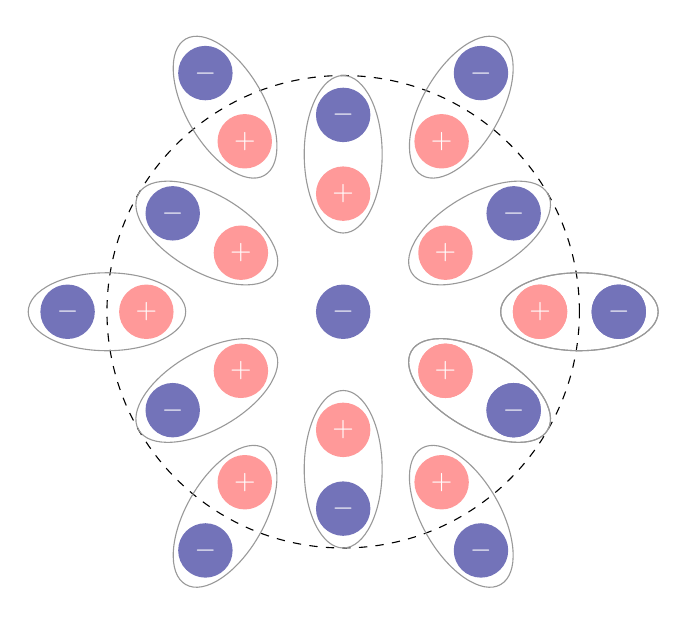
\begin{tikzpicture}
    \node[circle,fill=NavyBlue!55,radius=0.8] (A) at (0,0) {\textcolor{white}{$\mathbf{-}$}};
    \draw[color=black, dashed] (A) circle (3cm);
    \pgfmathsetmacro\n{6}
    \foreach \i in {0,...,\n} {
        \pgfmathsetmacro\r{\i*(360/\n)}
        \node[ellipse,draw=black!40,minimum height=2cm ,minimum width=0.99cm, rotate=\r+90] (n-\i) at (\r:3cm) {};
        \node[circle,fill=red!40,radius=0.8] (n-\i) at (\r:2.5cm) {\textcolor{white}{$\mathbf{+}$}};
        \node[circle,fill=NavyBlue!55,radius=0.8] (n-\i) at (\r:3.5cm) {\textcolor{white}{$\mathbf{-}$}}; %antes era blue!40

        \pgfmathsetmacro\R{\i*(360/\n)-30}
        \node[ellipse,draw=black!40,minimum height=2cm ,minimum width=0.99cm, rotate=\R+90] (n-\i) at (\R:2cm) {};
        \node[circle,fill=red!40,radius=0.8] (n-\i) at (\R:1.5cm) {\textcolor{white}{$\mathbf{+}$}};
        \node[circle,fill=NavyBlue!55,radius=0.8] (n-\i) at (\R:2.5cm) {\textcolor{white}{$\mathbf{-}$}};
        
    }
\end{tikzpicture}

\end{document}